\documentclass[../../thesis.tex]{subfiles}
\graphicspath{{./resources/} }
\begin{document}

\section{Optimizations}

\subsection{Stepwise Influence}\label{sec:optimization:stepwise_influence}

In \autoref{sec:group_sampling:influence_model} we created a model of a system by
taking the average value a feature has across groupings. In our example in \autoref{tab:group_sampling:feature_influence}
we were already able to see a problem \citet{saltelli2008global} described with group sampling. Features that
share a group with an influential feature look more influential than they truly are. \Citeauthor{saltelli2008global}
describe a way to determine the influence more accurately by determining the influence of a single parameter at a time.

The idea is to remove the influence an influential feature has before determining the influence of the next influential feature.
We can do this in two steps, for each feature we want to determine the influence for. First, we need to find the most influential
feature we have in our data. Then we have to estimate its influence and remove it from our data.

If we look at \autoref{tab:group_sampling:feature_influence} we can use the average measurements of a feature to identify the
most influential. But, we have to be aware, that the average of the measurements still includes the baseline performance.
By simply taking the highest measurement, we could end up picking the wrong feature, if, for example, the influential feature has
a negative effect on the measurement. We want to pick the outlier value of the average feature measurements.
One way to do this is to pick the feature where the average measurement is the furthest away from the average of all measurements.
In \autoref{tab:optimization:feature_influence} we can see, the average of all average measurements would be approximately $11.8$,
giving us $F_6$ as our outlier.

With the feature identified, we can remove it from our data. We estimate the influence of the feature the same way as previously, by taking
the average of all its measurements. By subtracting the value from all measurements where the feature was part of the group, we can get
a better estimate of the influence the rest of the features have. Then we remove the influential feature from our data
and proceed with identifying the next influential feature.
An example of this procedure can be found in \autoref{tab:optimization:feature_influence}.
We identified $F_6$ as our most influential feature and removed it and its influences in other groups from the data.
$F_6$ shared a group with $F_5$ and $F_3$ and after removing the estimated influence of $F_6$,
both do not look as influential as in \autoref{tab:group_sampling:feature_influence}.

In each round, we identify the influence of one feature. With the influences of the features determined that way, we can build our
model the same way as previously, but instead of using $I_n$ in \autoref{eq:group_sampling:intercept} and \autoref{eq:group_sampling:coefficient}
we use the values determined by our stepwise analysis.

\begin{table}[h]
  \caption{ Stepwise influence calculation }
  \begin{center}
    \begin{tabular}{ccc|c|cccccc|cccccc}\toprule
      $G_1$                 & $G_2$ & $G_3$ & $R$  & $F_1$ & $F_2$         & $F_3$         & $F_4$ & $F_5$ & $F_6$ & $F_1$ & $F_2$ & $F_3$ & $F_4$ & $F_5$ & $F_6$ \\ \midrule
      1                     & 0     & 0     & 3    & 1     & 1             & 0             & 0     & 0     & 0     & 3     & 3     &       &       &       &       \\
      0                     & 1     & 0     & 6    & 0     & 0             & 1             & 1     & 0     & 0     &       &       & 6     & 6     &       &       \\
      0                     & 0     & 1     & 28   & 0     & 0             & 0             & 0     & 1     & 1     &       &       &       &       & 1,5   &       \\ \midrule
      1                     & 0     & 0     & 2    & 1     & 0             & 0             & 1     & 0     & 0     & 2     &       &       & 2     &       &       \\
      0                     & 1     & 0     & 7    & 0     & 1             & 0             & 0     & 1     & 0     &       & 7     &       &       & 7     &       \\
      0                     & 0     & 1     & 25   & 0     & 0             & 1             & 0     & 0     & 1     &       &       & -1,5  &       &       &       \\ \midrule
      \multicolumn{10}{l}{} & 2,5   & 5     & 2,25 & 4     & \textbf{4,25} & \textbf{26,5}                                                                         \\ \midrule
    \end{tabular}
  \end{center}\label{tab:optimization:feature_influence}%
\end{table}

\subsection{Feature coverage}\label{sec:optimization:feature_coverage}

In this work, we use an SAT-solver to create valid configurations.
We can see the effects of it in \autoref{fig:group_sampling:samples}.
Off-the-shelf SAT-solvers tend to find locally clustered solutions \cite{kaltenecker2019distance}.
The repeating patterns in our samples are a result of it. The SAT-solver finds a solution
to our constraints by changing as few variables as possible.
Since at the beginning of each grouping, the constraints the solver has are similar,
the SAT-solver gives a similar solution. This prevents us from making meaningful groupings since
features regularly share the same group.

We adapt the distance-based sampling strategy introduced by \citet{kaltenecker2019distance} to
help in creating more diverse groups. We use the Hamming distance as shown in \autoref{eq:group_sampling:creation_of_groups:hamming:hamming_distance}
as our distance metric and the uniform distribution as our probability distribution.
Instead of measuring the distance from the origin, we measure the distance from the first group of the
previously created grouping.

In detail, at the start of each grouping, we randomly pick a distance from the first group created
in the previous grouping. We then set the distance as a constraint for our SAT-solver to avoid 
getting a similar first group. The following created groups are always dependent on the first group 
since they need to be distinct from each other. This way the groups created during each grouping do
not follow a pattern of minimal change.



\begin{figure}[htp]
  \begin{center}
    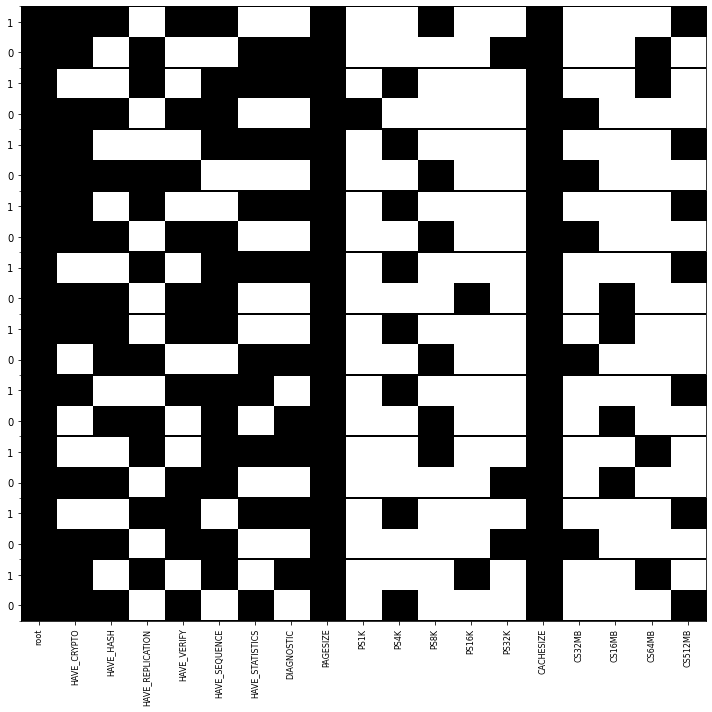
\includegraphics[width=0.49\textwidth]{sampling_distribution/gs_hamming_distance_optimization.png}
    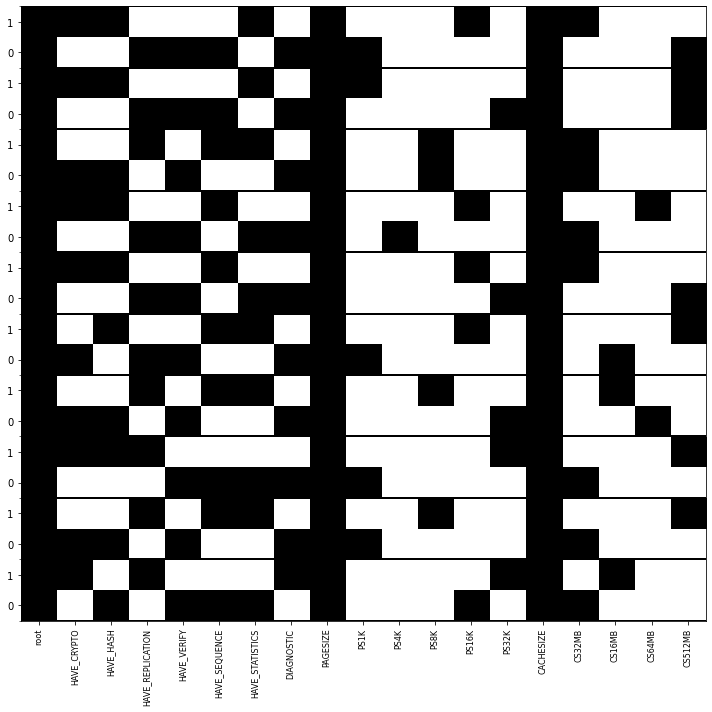
\includegraphics[width=0.49\textwidth]{sampling_distribution/gs_mutex_distance_optimization.png}
  \end{center}

  \caption[Group Sampling - Samples - Optimized]{
    Samples generated on the BerkeleyDB Dataset by both variations with distance based group optimization.
    \textbf{Left:}  Group Sampling - Hemming Distance - Group Size 2 - Groupings 10
    \textbf{Right:} Group Sampling - Independent features - Group Size 2 - Groupings 10
  }\label{fig:a}
\end{figure}



\end{document}


